\section{Metodologia}

\subsection{Termoscópio de Galileu}
O experimento foi realizado com um frasco de vidro conectado a um tubo capilar inserido em um recipiente contendo líquido corante. O frasco foi parcialmente submerso no líquido e após um dos participantes envolver o recipiente com a mão foi possível a observação do deslocamento da coluna líquida no tubo. A montagem está ilustrada na \cref{fig:termoscopio}.

\begin{figure}[H]
    \centering
    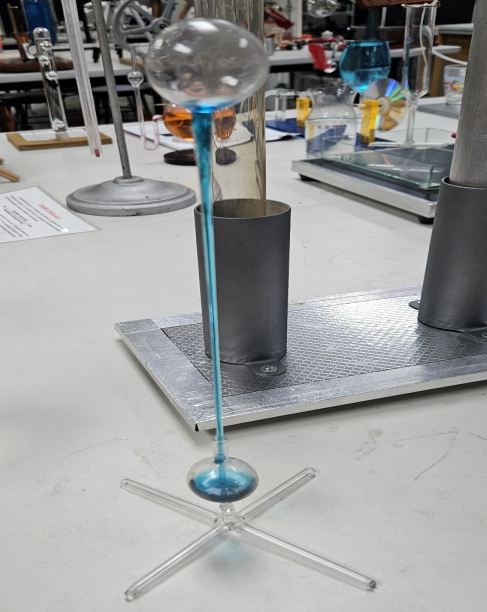
\includegraphics[width=0.35\linewidth]{fig/termoscopio.png}
    \caption{Montagem experimental do termoscópio de Galileu realizada em laboratório. A imagem mostra o frasco de vidro conectado a um tubo capilar parcialmente submerso em um recipiente com líquido corante. Fonte: fotografia tirada pelo monitor Pedro.}
    \label{fig:termoscopio}
\end{figure}

\subsection{Termômetro de Galileu}
O aparato experimental consistiu em um cilindro de vidro preenchido com líquido transparente, contendo cápsulas esféricas calibradas de densidade próxima. As cápsulas foram observadas em repouso, e sua posição vertical dentro do tubo foi registrada. A \cref{fig:termometro} apresenta a montagem.

\begin{figure}[H]
    \centering
    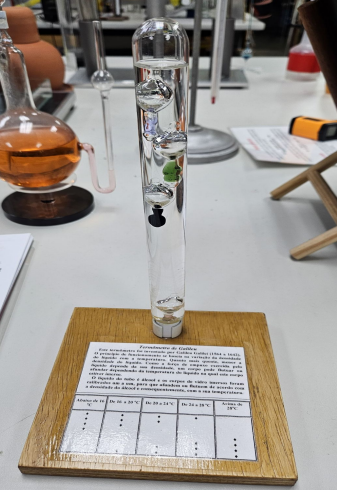
\includegraphics[width=0.25\linewidth]{fig/termometro.png}
    \caption{Termômetro de Galileu utilizado durante a aula. O dispositivo contém cápsulas esféricas calibradas, submersas em um líquido transparente dentro de um cilindro de vidro. Fonte: registro fotográfico feito pelo monitor Pedro.}
    \label{fig:termometro}
\end{figure}

\subsection{Higrômetro (Psicrômetro)}
Foram utilizados dois termômetros idênticos, sendo um mantido com o bulbo seco e o outro com o bulbo envolto em gaze úmida. Ambos foram posicionados lado a lado em suporte comum. Após exposição ao ar ambiente por tempo determinado, foram anotadas as temperaturas dos dois termômetros e os dados foram correlacionados por meio de uma tabela presente na estrutura entre os termômetros. A montagem pode ser visualizada na \cref{fig:psicrometro}.

\begin{figure}[H]
    \centering
    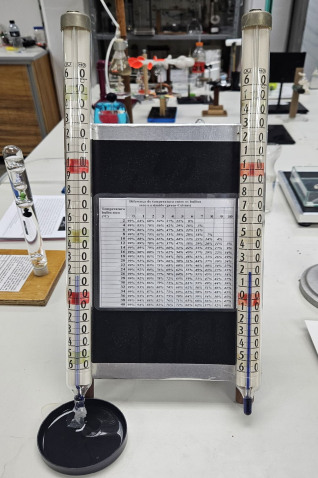
\includegraphics[width=0.30\linewidth]{fig/psicrometro.png}
    \caption{Psicrômetro montado sobre suporte metálico, com os dois termômetros fixados lado a lado. O bulbo de um dos termômetros está envolvido por gaze umedecida. Fonte: fotografia registrada pelo monitor da disciplina, Pedro.}
    \label{fig:psicrometro}
\end{figure}

\subsection{Anel de Gravesande}
Foi utilizada uma esfera metálica acoplada a uma haste, e um anel metálico com diâmetro interno ligeiramente maior que o da esfera em temperatura ambiente. A esfera foi inicialmente posicionada sobre o anel. Em seguida, foi aquecida com uma fonte térmica até não mais atravessar o anel. Após resfriamento natural, o teste de passagem foi repetido. A montagem é mostrada na \cref{fig:gravesande}.

\begin{figure}[H]
    \centering
    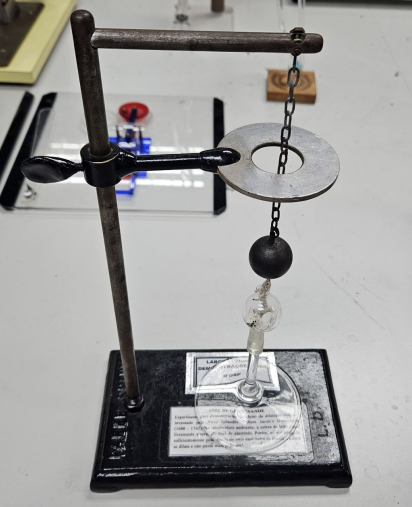
\includegraphics[width=0.30\linewidth]{fig/gravesande.png}
    \caption{Montagem do experimento do Anel de Gravesande. A imagem mostra a esfera metálica acoplada a uma haste após passar pelo anel metálico e o dispositivo que foi utilizado como fonte de calor durante o experimento. Fonte: fotografia capturada pelo monitor Pedro.}
    \label{fig:gravesande}
\end{figure}

\subsection{Par Bimetálico}
A montagem experimental consistiu em uma lâmina bimetálica fixa em uma extremidade e livre na outra. A lâmina foi aquecida com uma chama direta e observou-se a mudança da sua posição durante todo o processo. A \cref{fig:bimetalico} apresenta o aparato utilizado.

\begin{figure}[H]
    \centering
    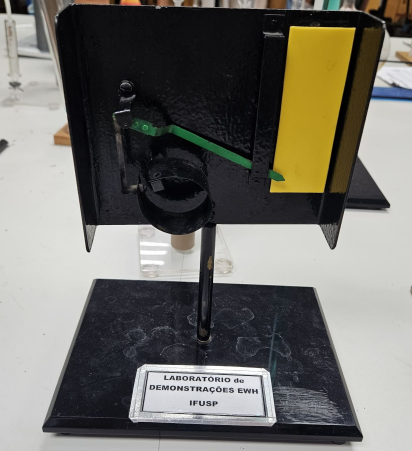
\includegraphics[width=0.35\linewidth]{fig/bimetalico.png}
    \caption{Lâmina bimetálica fixada em suporte metálico. A fonte de calor utilizada no experimento não consta na imagem. Fonte: imagem feita pelo monitor da diciplina, Pedro.}
    \label{fig:bimetalico}
\end{figure}
